\subsection{Identity-Transformation Algorithms}
\label{subsec:overview}

We design identity transformations on an elliptic curve $\mathbb{E}$,
and Table \ref{tbl:notations-protocol} lists the notations.
%The subscript $j$ and/or superscript $i$ may be omitted if there is no ambiguity.


\begin{table}[tb]
\footnotesize
    \caption{Notations used in the \usso\ protocol}
    \centering
%    \begin{tabular}{|c|c|c|}
    \begin{tabular}{|p{0.93cm}|p{6.71cm}|} \hline
    {\textbf{Notation}} & {\textbf{Description}} \\ \hline
    {$\mathbb{E}$, $G$, $n$} & {$\mathbb{E}$ is an elliptic curve over a finite field $\mathbb{F}_q$. $G$ is a base point (or generator) on $\mathbb{E}$, and the order of $G$ is a prime number $n$.} \\ \hline
    {$ID_{U_i}$} & {$ID_U = u \in \mathbb{Z}_n$ is the $i$-th user's unique identity at the IdP, which is known only to the IdP.} \\ \hline
   {$ID_{RP_j}$} & {$ID_{RP} = [r]G$ is the $j$-th RP's unique identity, which is publicly known; $r \in \mathbb{Z}_n$ is known to \emph{nobody}.} \\ \hline
    {$t$} & {$t \in \mathbb{Z}_n$ is a user-selected random integer in each login; $t$ is shared with the target RP and kept unknown to the IdP.} \\ \hline
    {$PID_{RP_j}^l$} & {$PID_{RP} = [t]{ID_{RP}} = [tr]G$ is the $j$-th RP's pseudo-identity, in the user's $l$-th login visiting this RP.} \\ \hline
    {$PID_{U_i,j}^l$} & {$PID_U = [{ID_U}]{PID_{RP}} = [utr]G$ is the $i$-th user's pseudo-identity, in the user's $l$-th login visiting the $j$-th RP.} \\ \hline
     {$Acct_{i,j}$} & {$Acct = [t^{-1}\bmod n]PID_{U} = [ID_U]ID_{RP} = [ur]G$ is the $i$-th user's locally-unique account at the $j$-th RP, publicly known.} \\ \hline
    {$SK$, $PK$} & {The IdP's private key and public key, used to sign and verify identity tokens and RP certificates.} \\ \hline
    {$Enpt_{RP_j}$} & {The $j$-th RP's endpoint for receiving the identity tokens.} \\ \hline
    {$Cert_{RP_j}$} & {The IdP-signed RP certificate binding $ID_{RP_j}$ and $Enpt_{RP_j}$.} \\ \hline
    \end{tabular}
    \label{tbl:notations-protocol}
\end{table}

\noindent {\bf $\boldsymbol{ID_{\boldsymbol{U}}}$, $\boldsymbol{ID_{\boldsymbol{RP}}}$ and $\boldsymbol{Acct}$.}
The IdP assigns a unique random integer $u \in \mathbb{Z}_n$ to a user (i.e., $ID_U = u$),
 and randomly selects unique $ID_{RP} = [r]G$ for a registered RP. % if it is a point on $\mathbb{E}$.
Here, $G$ is a base point on $\mathbb{E}$ of order $n$, and $[r]G$ denotes the addition of $G$ on the curve $r$ times.

$Acct = \mathcal{F}_{Acct\ast}(ID_U, ID_{RP_j})= [ID_U]ID_{RP_j} =[ur_j]G$ is automatically assigned 
        to a user at every RP,
and a user's accounts at different RPs are inherently different and unlinkable.

\noindent {\bf $\boldsymbol{ID_{\boldsymbol{RP}}}$-$\boldsymbol{PID_{\boldsymbol{RP}}}$ Transformation.} In each login, a user selects a random number $t \in \mathbb{Z}_n$ to calculate $PID_{RP}$.
\begin{equation}
PID_{RP} = \mathcal{F}_{PID_{RP}}(ID_{RP}) = [t]{ID_{RP}} = [tr]G
\label{equ:PIDRP}
\end{equation}


%In each login, the user selects $t$ and shares it with the RP to negotiate $PID_{RP}$. 
%--removed due to double-check discussion
%It makes no difference if the RP selects $t$ randomly and sends it to the user, as long as both of them calculate $PID_{RP}$ \emph{independently} and check if the received $PID_{RP}$ is equal to the calculated one.

\noindent {\bf $\boldsymbol{ID_U}$-$\boldsymbol{PID_U}$ Transformation.}
On receiving an identity-token request for $PID_{RP}$ from a user identified as $ID_U$, the IdP calculates $PID_{U}$ as below.
\begin{equation}
PID_{U} = \mathcal{F}_{PID_U}(ID_U, PID_{RP}) =
  [{ID_U}]{PID_{RP}} = [utr]G
 \label{equ:PIDU}
\end{equation}


\noindent {\bf $\boldsymbol{PID_U}$-$\boldsymbol{Acct}$ Transformation.}
The user sends $t$ to the target RP as a trapdoor to derive her account.
After verifying a token that encloses $PID_U$ and $PID_{RP}$, it calculates $Acct$ as follows.
\begin{equation}
Acct = \mathcal{F}_{Acct}(PID_{U})
   = [t^{-1} \bmod n]PID_{U}
   \label{equ:Account}
\end{equation}
From Equations \ref{equ:PIDRP}, \ref{equ:PIDU}, and \ref{equ:Account}, it is derived that
\begin{equation}
   Acct =  [t^{-1}utr]G = [ur]G = \mathcal{F}_{Acct\ast}(ID_U, ID_{RP})
   \label{equ:AccountNotChanged}
\end{equation}


With the help of $t$, the visited RP derives an identical account for a user in her different logins. It is exactly the user's \emph{permanent} account at this RP.

A user's identity $u$ is unknown to all entities except the honest IdP; otherwise, colluding RPs could calculate $[u]ID_{RP_j}$s for any known $u$ and link these accounts.
Meanwhile, $ID_{RP} = [r]G$ and $Acct = [ID_U]ID_{RP}$ are publicly-known,
 but $r$ is always kept secret;
otherwise, two colluding RPs with $ID_{RP_j} = [r]G$ and $ID_{RP_{j'}} = [r']G$ could link a user's accounts by checking whether $[r']Acct_j$ is equal to $[r]Acct_{j'}$ or not.

\subsection{The Designs Specific for Web Applications}
\label{sec:web-design}

%The user's operations, e.g., request redirection, authorization, and token forwarding, are performed by user agents, such as a browser for web applications.

In commonly-used SSO protocols \cite{OpenIDConnect,rfc6749, SAML, SAMLIdentifier},
an IdP needs to know the visited RP to ensure confidentiality of identity tokens. For instance, in OIDC services with redirect UX, an RP's endpoint to receive tokens is stored as the \texttt{redirect\_uri} parameter at the IdP.
The IdP employs HTTP 302 redirection to send tokens to the RP, by setting this parameter as the target URL in the HTTP response to a user's identity-token request \cite{OpenIDConnect}.
  % so the user agent (i.e., browser) forwards it to the designated RP.
Alternatively, in an OIDC system with pop-up UX  \cite{dimvaLiM16,GoogleIdIntegrate,uber}, the user-i script confirms the target RP's origin with the IdP, and then forwards tokens to the user-r script restricted by this origin.

In \usso\ the IdP does not know about the visited RP, requiring a user agent by itself to calculate $PID_{RP}$ and forward identity tokens to the RP.
We implement \usso\ compatibly in OIDC services with pop-up UX \cite{GoogleIdIntegrate,uber},
 and the user-agent functions are also implemented by the two scripts,
%        i.e., the user-i script and the user-r script,
    downloaded from the IdP and the visited RP, respectively.
%The scripts are responsible for communicating with the origin web servers and also the cross-origin communications within the browser.
% as most browsers do in secure OIDC settings \cite{de2014oauth,GoogleIdIntegrate}.
%\footnote{The user-i script is recommended in OIDC services for an in-context user experience of attribute authorization \cite{GoogleIdIntegrate,uber}, so the authorization of user attributes is also implemented through this user-i script in \usso.}
The user-i script is necessary in \usso\ and then it cannot be integrated in OIDC services with redirect UX, 
because the user-r script could leak its origin to the IdP web server (i.e., break IdP untraceability) due to the automatic inclusion of an HTTP \texttt{referer} header in HTTP requests it sends.


In original OIDC systems with pop-up UX,
    the user-i script implements attribute authorization and token receiving,
        while the user-r script receives token requests from the visited RP and forwards tokens to the target RP.
We improve these scripts as below to further support identity transformations.
In each login, the user-r script prepares $ID_{RP}$ and $Enpt_{RP}$ %for the user-i script,
 through an RP certificate, returned in the token request. %It binds the RP's identity and endpoint. %(i.e., $ID_{RP}$ and $Enpt_{RP}$).
The user-r script sends the certificate to the user-i script, which verifies it to extract $ID_{RP}$ and $Enpt_{RP}$.
Note that in \usso\ a user configures nothing locally for the IdP's public key is set in the user-i script, like in other popular SSO systems \cite{OpenIDConnect, rfc6749, SAML, SAMLIdentifier}.
Then, within a browser the user-i script calculates $PID_{RP} = [t]ID_{RP}$ based on $ID_{RP}$ extracted from the verified RP certificate, % that binds $ID_{RP}$ and $Enpt_{RP}$.
%This should be conducted by an \emph{honest} script that obtains $ID_{RP}$ correctly
%    and does not leak $t$, from which it could calculate $ID_{RP} = [t^{-1}\bmod n]PID_{RP}$.
 %otherwise, it could directly leak the RP's domain to the IdP.\footnote{To eliminate this assumption, we can implement the user-agent functions with trusted browser extensions, which are installed before a user visits RPs.}
to request a token for $PID_{RP}$.
On receiving an identity-token request, the IdP web server checks the included \texttt{referer} header to ensure it is sent by the user-i script.


After receiving a token from the IdP, the user-i script needs to ensure the user-r script will forward the token to $Enpt_{RP}$ %, which is bound with $ID_{RP}$
specified in the verified RP certificate.
As the communications between scripts occurs within COTS browsers using the \verb+postMessage+ HTML5 API, %To avoid the honest user sending the identity token to an adversary,
the \verb+postMessage+ targetOrigin mechanism \cite{postm-targeto} restricts the recipient. %(i.e., the RP script).
When the user-i script sends messages, the recipient's origin is set as a parameter, e.g., \verb+postMessage(tk, 'https://RP.com')+, including the protocol (i.e., \verb+https+), the domain (i.e., \verb+RP.com+), and a port if applicable.
Only the script downloaded from this targetOrigin is a legitimate recipient.
This design is commonly used to correctly forward tokens in popular OIDC systems \cite{SPRESSO,MITREid,BrowserID,de2014oauth,OpenIDConnect}.

%The \emph{RP certificates} deals with the problem of mapping an identity proof with its targeting RP.
%That is, the IdP script derives the RP's $ID_{RP}$ and origin from the RP certificate, while the $PID_{RP}$ is generated with this $ID_{RP}$. Thus, the IdP script always knows the targeting RP of identity proof, therefore, the \verb+postMessage+ mechanism can guarantee that the identity proof would not be sent to the adversary.


Besides, when a user attempts to visit an RP in \usso\ (and OIDC systems with pop-up UX), the RP window downloads the user-r script, which in turn ``pops up'' a new browser window to access the IdP and download the user-i script.
To prevent referer leakage during this access, we need to ensure the HTTP request does not carry a \texttt{referer} header, which reveals the visited RP's domain to the IdP server.\footnote{In original OIDC services with pop-up UX this leakage commonly exists, but does not matter because such services are not designed to prevent IdP-based login tracing.} %Generally, when a browser window visits another website not belonging to its opener's origin, the HTTP request to this website automatically carries a \texttt{referer} header (i.e., the opener's origin). Such an HTTP header leaks the visited RP's domain to the IdP.
Fortunately, in \usso\ this pop-up is an HTTP redirection from the new window to the IdP (Steps 1.2-1.3 in Figure \ref{fig:process}), but not a direct visit.
The HTTP redirection response from the RP server includes a \texttt{referrer-policy=no-referrer} header, which ensures that the HTTP request to access the IdP carries no \texttt{referer} header.
This method is specified by W3C \cite{referer_policy} and widely supported. We have tested it in various browsers such as Chrome, Safari, Edge, Opera, and Firefox, and confirmed no referer leakage.

\begin{figure*}[htb]
  \centering
  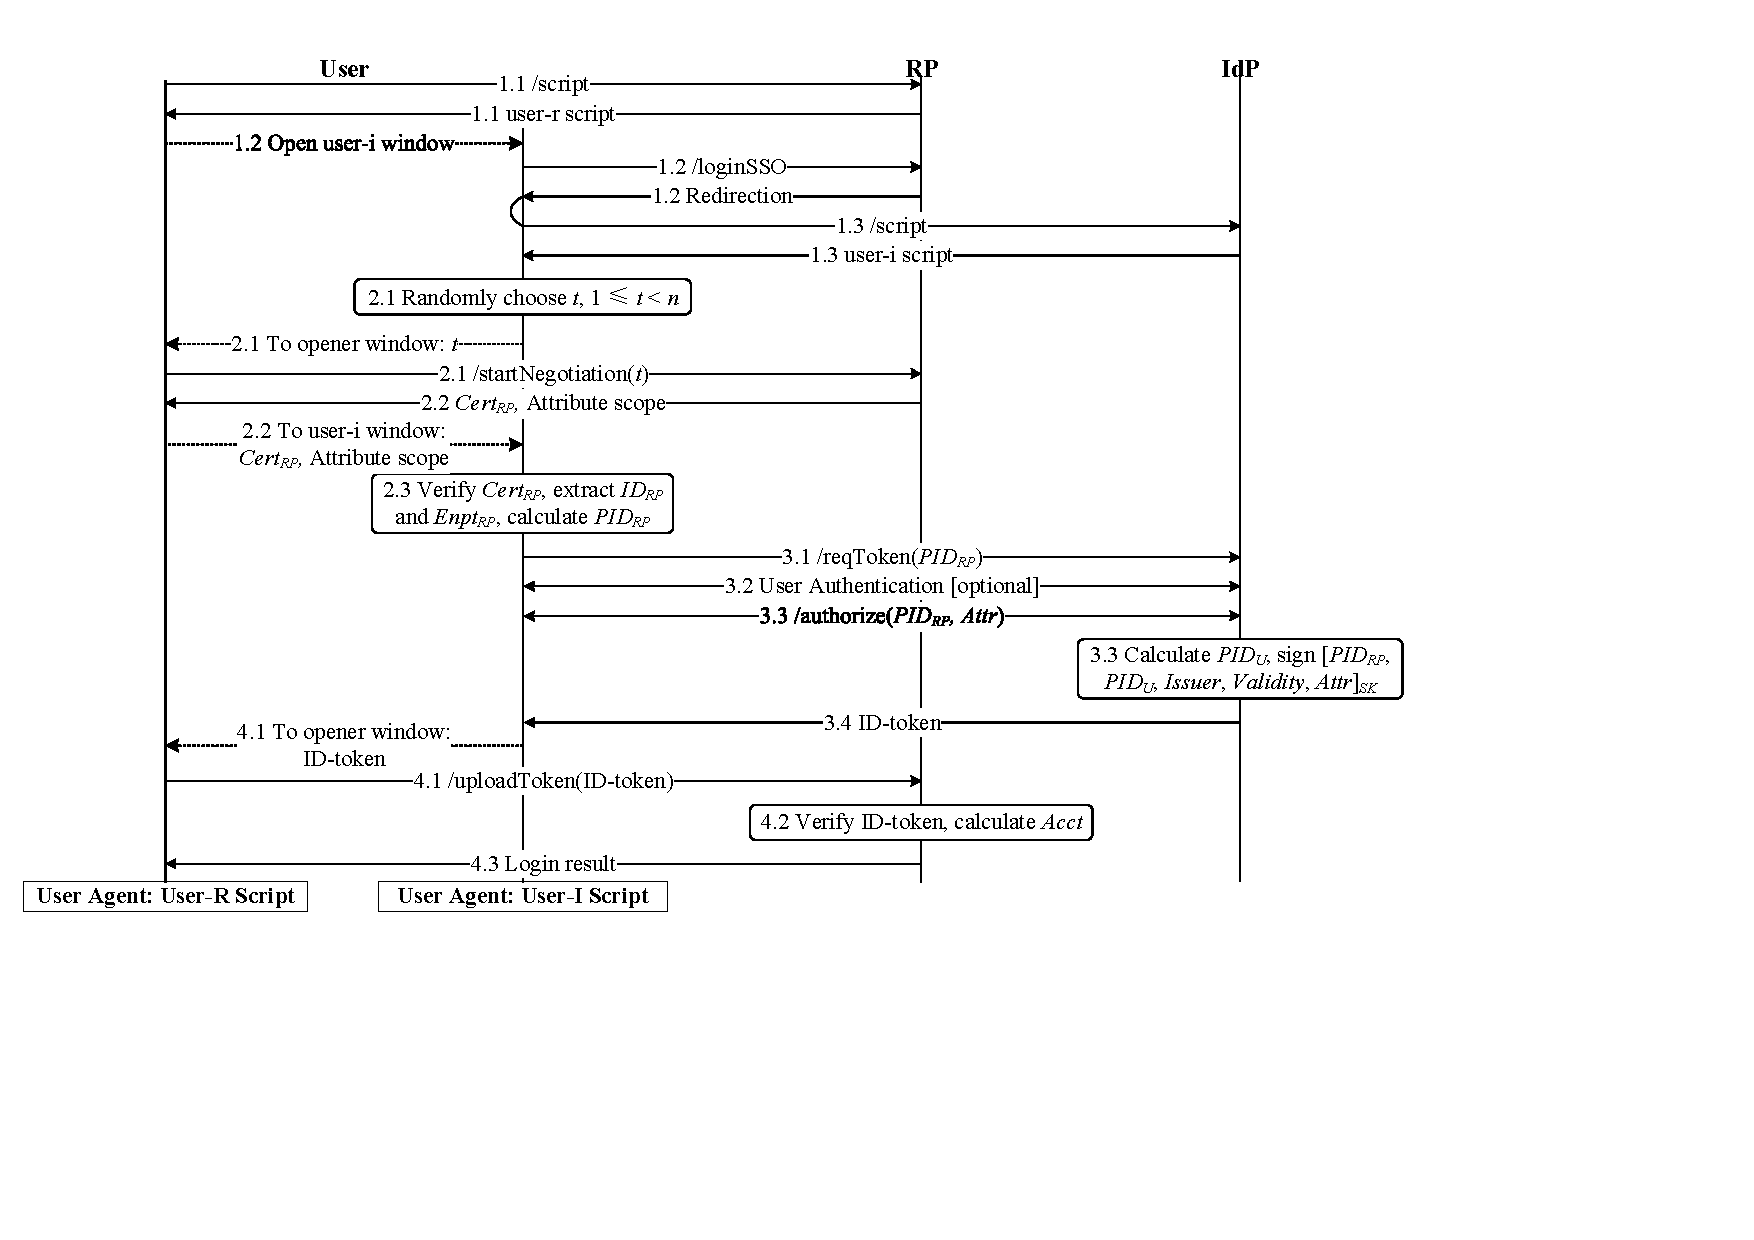
\includegraphics[height=0.491\textheight]{fig/process-js.pdf}
  \caption{The SSO login flow of \usso}
  \label{fig:process}
\end{figure*}



\subsection{The \usso\ protocol}
\label{implementations}

\noindent \textbf{System Initialization.}
$\mathbb{E}$, $G$ and $n$ are set up and publicly published.
An IdP generates a key pair ($SK$, $PK$) to sign and verify identity tokens and RP certificates.
%The IdP keeps $SK$ secret, and $PK$ is publicly known.

\vspace{1mm}
\noindent\textbf{RP Registration.}
Each RP registers itself at the IdP to obtain $ID_{RP}$ and its RP certificate $Cert_{RP}$ as follows.
This registration may be conducted by face-to-face means.
\vspace{-\topsep}\begin{enumerate}
\setlength{\topsep}{0pt}
\setlength{\partopsep}{0pt}
\setlength{\itemsep}{0pt}
\setlength{\parsep}{0pt}
\setlength{\parskip}{0pt}
\item[1.]
An RP pre-installs $PK$ by trusted means.
It sends a registration request, including the endpoint to receive identity tokens and other information.
\item[2.]
After examining the request,
the IdP randomly selects $r \in \mathbb{Z}_n$
        and assigns a \emph{unique} point $[r]G$ to the RP as its identity.
Note that $r$ is not processed any more and then known to \emph{nobody}
 due to the elliptic curve discrete logarithm problem (ECDLP).
%random number $r \in [1,n)$ until $ID_{RP} = [r]G$ is unique.
 %   but $r$ is kept unknown to the RP.
The IdP then signs $Cert_{RP} = [ID_{RP}, Enpt_{RP}, *]_{SK}$,
     where $[\cdot]_{SK}$ is a message signed using $SK$ and $*$ is supplementary information such as the RP's common name.
\item[3.]
The RP verifies $Cert_{RP}$ using $PK$, and accepts $ID_{RP}$ and $Cert_{RP}$ if they are valid.
\end{enumerate}

%\vspace{0.5mm}
\noindent\textbf{User Registration.}
%Each user registers once at the IdP. 
Each user sets up her unique username and the corresponding credential for the IdP.
The IdP assigns
a unique random identity $ID_U = u\in \mathbb{Z}_n$ to the user.

It is required that $ID_U$ is known \emph{only} to the IdP.
$ID_U$ is used only by the IdP \emph{internally},
 not enclosed in any message.
%so a user inputs her username in the authentication to the IdP and $ID_U$ is processed only by the IdP internally.
For example, a user's identity is generated and always restored by hashing her username concatenated with the IdP's private key.
Then,
 $ID_U$ is never stored in hard disks,
 and protected almost the same as the IdP's private key
because it is \emph{only} used to calculate $PID_{U}$ as the IdP is signing a token binding $PID_{U}=
  [{ID_U}]{PID_{RP}}$.

\vspace{1mm}
\noindent\textbf{SSO Login.} 
A registered user may log into any registered RP,
    after authenticated herself to the IdP.
A login flow %is typically launched through a browser,
%when a user attempts to visit an RP. It
involves four steps: script downloading, RP identity transformation, identity-token generation, and $Acct$ calculation. In Figure \ref{fig:process}, the IdP's and RP's operations are connected by two vertical lines, respectively. The user operations are split into two groups in different browser windows by vertical lines, one communicating with the IdP and the other with the RP. Solid horizontal lines indicate messages exchanged between a user and the IdP (or the RP), while dotted lines represent \verb+postMessage+ invocations between two scripts (or browser windows) within a browser.


\vspace{1mm}
\noindent 1. {\em Script Downloading.}
The browser downloads user-agent scripts from the visited RP and the IdP as below.
\vspace{-\topsep}
\begin{itemize}
\setlength{\topsep}{0pt}
\setlength{\partopsep}{0pt}
\setlength{\itemsep}{0pt}
\setlength{\parsep}{0pt}
\setlength{\parskip}{0pt}
\item[1.1]
When requesting any protected resources at the RP, the user downloads the user-r script.
\item[1.2]
The user-r script opens a window in the browser to visit the RP's login path, which is then redirected to the IdP.
\item[1.3]
The redirection to the IdP downloads the user-i script.
\end{itemize}


\noindent 2. {\em RP Identity Transformation.}
The user and the RP negotiate $PID_{RP} = [t]{ID_{RP}}$.
\vspace{-\topsep}
\begin{itemize}
\setlength{\topsep}{0pt}
\setlength{\partopsep}{0pt}
\setlength{\itemsep}{0pt}
\setlength{\parsep}{0pt}
\setlength{\parskip}{0pt}
\item[2.1] The user-i script chooses a random number $t \in \mathbb{Z}_n$ and sends it to the user-r script through \verb+postMessage+. The user-r script then forwards $t$ to the RP.
\item[2.2] The RP verifies if the received $t$ is an integer in $\mathbb{Z}_n$, and
%Upon receiving $t$, the RP verifies $1 \leq t < n$ and %calculates $PID_{RP}$.
%To acknowledge the negotiation of $PID_{RP}$, The RP
replies with $Cert_{RP}$ and the scope of requested attributes, forwarded by the user-r script to the user-i script.  % through \verb+postMessage+.
\item[2.3] The user-i script verifies $Cert_{RP}$, extracts $ID_{RP}$ and $Enpt_{RP}$ from $Cert_{RP}$, and calculates $PID_{RP}=[t]{ID_{RP}}$.

\end{itemize}


%\vspace{1mm}
\noindent 3. {\em Identity-Token Generation.}
The IdP calculates $PID_U = [ID_U]{PID_{RP}}$ and signs an identity token as follows. % The processes are as follows.
\vspace{-\topsep}
\begin{itemize}
\setlength{\topsep}{0pt}
\setlength{\partopsep}{0pt}
\setlength{\itemsep}{0pt}
\setlength{\parsep}{0pt}
\setlength{\parskip}{0pt}
\item[3.1]
The user-i script sends an identity-token request for $PID_{RP}$ on behalf of the user. %and the user attributes.
 %by checking whether this user is authenticated by IdP.

\item[3.2] The IdP authenticates the user, if not authenticated yet.

\item [3.3]
The user-i script displays the RP's common name,
 locally obtains the user's authorization for the requested attributes,
 and then sends the scope of the authorized attributes.
The IdP checks that $PID_{RP}$ is a point on $\mathbb{E}$,
calculates $PID_U = [ID_U]{PID_{RP}}$, and signs $[PID_{RP}, PID_U, Issuer, Validity, Attr]_{SK}$, where $Issuer$ is the IdP, $Validity$ indicates the validity period, and $Attr$ contains the authorized user attributes.
\item[3.4] The IdP replies with the identity token to the user-i script.
\end{itemize}

%\vspace{1mm}
\noindent 4. {\em $Acct$ Calculation.}
The RP receives the identity token and allows the user to log in.
\vspace{-\topsep}
\begin{itemize}
\setlength{\topsep}{0pt}
\setlength{\partopsep}{0pt}
\setlength{\itemsep}{0pt}
\setlength{\parsep}{0pt}
\setlength{\parskip}{0pt}
\item [4.1]
The user-i script forwards the identity token to the user-r script,
    which then sends it to the RP through $Enpt_{RP}$.
\item[4.2] The RP verifies the signature and the validity period of the token 
%Then, the RP extracts $PID_{RP}$ from the token, checks if it equals $[t]ID_{RP}$,
and calculates $Acct = [t^{-1}]{PID_U}$.

\item [4.3] The RP allows the user to log in as $Acct$.

\end{itemize}


If any verification fails, this flow will be terminated immediately.
For example, the user halts it when receiving an invalid $Cert_{RP}$.
The IdP rejects an identity-token request in Step 3.3 if the received $PID_{RP}$ is not a point on $\mathbb{E}$, and the RP rejects a token in Step 4.2 if the signature is invalid. 

%%%%%%%%%%%%%%%%%%%%%%%%%%%%%%%%%%%%%%%%%%%%%%%%%%%%%%%%%%
% u泄露,则RP有必要比较!否则,就会伤害security。
%or the enclosed $PID_{RP}$ is not equal to $[t]ID_{RP}$.
%%%%%%%%%%%%%%%%%%%%%%%%%%%%%%%%%%%%%%%%%%%%%%%%%%%%%%%%%%
% 分析结论是:
% 现有的简化协议(RP不比较$PID_{RP}$是否相等),则:
% 当u不泄露,u的security和privacy都没有问题;
% 当u泄露,u的security和privacy都有问题。
%
% 改进协议(RP比较$PID_{RP}$是否相等),则:
% 当u不泄露,u的security和privacy都没有问题;
% 当u泄露,u的security没有问题,u的privacy有问题。
%%%%%%%%%%%%%%%%%%%%%%%%%%%%%%%%%%%%%%%%%%%%%%%%%%%%%%%%%%

\subsection{Compatibility with OIDC}
\label{subsec:compatible}

An OIDC system works in two alternative modes \cite{dimvaLiM16,GoogleIdIntegrate,uber,de2014oauth}:
 pop-up UX with two web scripts, and redirect UX with only the user-r script.
\usso\ only works in OIDC systems with pop-up UX. %(i.e., the communication flows among the IdP, the browser and the visited RP are identical),
  %  while the downloaded scripts are modified to support identity transformations.
%Both \usso\ and OIDC work with COTS browsers. %Among the four steps of the login flow
%
When a user attempts to visit an RP in \usso,
        a user agent is prepared by two scripts in the \emph{script downloading} step.
These scripts are downloaded, % following the same flow 
like in OIDC systems with pop-up UX.
%In \usso\ two scripts implement the verifications of RP certificates 
%  and the user operations of identity transformations, in addition to attribute authorization and token receiving by the user-i script and token forwarding by the user-r script in original OIDC services.
%
%\usso\ employs web scripts to hide the RP's endpoint from the IdP, while securely forwarding identity tokens to the RP through $Enpt_{RP}$ extracted from the signed RP certificate.
%Thus, the IdP cannot set \texttt{redirect_uri} in the HTTP responses, which is different from OIDC where HTTP redirections are used to implement these communications.
%

The \emph{RP identity transformation} step in \usso\ take place within a browser,
            and the RP responds with its certificate after receiving $t$.
The RP response is constructed following the standard format of OIDC requests \cite{dimvaLiM16},
    but then processed by the user-i script to remove any information leaking the RP's identity.
%which can be viewed as a supplementary access to static resources on the RP server.
%The operations in the $PID_{RP}$ registration are almost identical to those in the RP Dynamic Registration of OIDC \cite{DynamicRegistration}, except that in OIDC the IdP assigns the RP's identity  while in UPPRESSO this (pseudo-)identity is generated by the registered entity. Besides, the $PID_{RP}$ registration has a validity period.

The operations of \emph{identity-token generation} in \usso\ are compatible with those in OIDC,
 because (\emph{a}) the calculation of $PID_U$ is actually a special method to generate PPIDs and (\emph{b}) $PID_{RP}$ can be viewed as a ``dynamic'' RP pseudo-identity
    so that \texttt{redirect\_uri} is missing in the responses by the IdP.
%
%Compared to the original OIDC protocol, \usso\ simplifies the IdP's operations in these two steps, while allowing ``dynamic'' RP pseudo-identities.
Finally, the operations of \emph{$Acct$ calculation} in \usso\ are identical to those in OIDC,
 because the calculation of $Acct$ is a mapping from the user pseudo-identity enclosed in tokens to a local account at the visited RP.

The compatibility is experimentally confirmed through our prototype implementation.
When we built the IdP prototype of \usso\ on top of MITREid Connect \cite{MITREid},
    only 23 lines of Java code are added:
        three lines to calculate $PID_U$ as a special PPID using Java cryptographic libraries,
    and 20 lines to support pop-up UX with identity transformations.
%    modify the method of forwarding identity tokens.
